\documentclass{beamer}
\usetheme[progressbar=frametitle,block=fill]{metropolis}           % Use metropolis theme

\usepackage[spanish]{babel}
\usepackage[utf8]{inputenc}
\uselanguage{spanish}
\languagepath{spanish}
\deftranslation[to=spanish]{Theorem}{Teorema}
\deftranslation[to=spanish]{theorem}{teorema}

\usepackage{tikz}


\title{Pruebas de Conocimiento Cero y sus Aplicaciones}
\date{\today}
\author{José Luis Cánovas Sánchez\\[3mm]\scriptsize Tutores:\\Antonio José Pallarés Ruiz\\Leandro Marín Muñoz}

\institute{Universidad de Murcia\\Facultad de Matemáticas}
\begin{document}
\maketitle

\begin{frame}
	\frametitle{Outline}
	\tableofcontents
\end{frame}

\section{Decision Problems}

\begin{frame}{Decision Problem}
	\begin{definition}[Decision Problem]
		General description of a task which depend on some parameters and which possible answers are in the set $\{True, False \}$.
	\end{definition}
	\begin{description}[Parameters]
		\item[Name] \textit{A characteristic name.}
		\item[Parameters] \textit{Arguments the problem depends on}.
		\item[Question] \textit{Question such the possible answers are} $True$ \textit{or} $False$.
	\end{description}
\end{frame}

\begin{frame}{Graph Isomorphism}
	\begin{description}[Parameters]
		\item[Name] Graph Isomorphism Problem (GI).
		\item[Parameters] Given two graphs $G_1 = (V_1, E_1)$ and $G_2 = (V_2, E_2)$ with $\mid V_1 \mid = \mid V_2 \mid = n$.
		\item[Question] Is there a permutation $\tau : V_1 \rightarrow V_2$ such that an edge $(u,v)\in E_1$ if and only if $(\tau (u),\tau (v)) \in E_2$?
	\end{description}



		
	\begin{center}
		% Define style for nodes
	\tikzstyle{every node}=[circle, draw, fill=black!50, inner sep=0pt, minimum width=4pt]
	%  Tutte's 8-cage
	\begin{tikzpicture}[thick,scale=0.5]
	% The following path utilizes several useful tricks and features:
	% 1) The foreach statement is put inside a path, so all the edges
	%    will in fact be a the same path.
	% 2) The node construct is used to draw the nodes. Nodes are special
	%    in the way that they are drawn *after* the path is drawn. This
	%    is very useful in this case because the nodes will be drawn on
	%    top of the path and therefore hide all edge joins.
	% 3) Simple arithmetics can be used when specifying coordinates.
	\draw \foreach \x in {0,36,...,324}
	{
		(\x:2) node {}  -- (\x+108:2)
		(\x-10:3) node {} -- (\x+5:4)
		(\x-10:3) -- (\x+36:2)
		(\x-10:3) --(\x+170:3)
		(\x+5:4) node {} -- (\x+41:4)
	};
	\end{tikzpicture}\quad
	\begin{tikzpicture}[thick,scale=0.5]
	\draw \foreach \x in {0,36,...,324}
	{
		(\x:2.5) node {}  -- (\x+108:2.5)
		(\x-10:4) node {} -- (\x+5:1)
		(\x-10:4) -- (\x+36:2.5)
		(\x-10:4) --(\x+170:4)
		(\x+5:1) node {} -- (\x+41:1)
	};
	\end{tikzpicture}
	\end{center}
\end{frame}


\begin{frame}{Hamiltonian Cycle \textsuperscript{NPC}}
\begin{description}[Parameters]
	\item[Name] Hamiltonian Cycle Problem (HC).
	\item[Parameters] Given graph $G=(V,E)$.
	\item[Question] Does there exist a Hamiltonian cycle in $G$?
\end{description}

\begin{center}
	\tikzstyle{every node}=[circle, draw, fill=black!50, inner sep=0pt, minimum width=8pt]
\begin{tikzpicture}[thick]
	\draw [line width=0.8mm,purple](120:2) -- (240:2) -- (0:2) -- (0:0) -- cycle;
	\draw (120:2) node {} -- (0:2) node {};
	\draw (0:0) node {} -- (240:2) node {};
\end{tikzpicture}
\end{center}

\end{frame}


\begin{frame}{Graph 3-colorability \textsuperscript{NPC}}

\begin{description}[Parameters]
	\item[Name] Graph 3-colorability Problem (G3C).
	\item[Parameters] Given graph $G=(V,E)$.
	\item[Question] Is there a function	$\phi : V \to \{1,2,3\}$ such that $\phi(u)\neq \phi(v) \quad \forall (u,v)\in E$?
\end{description}

\begin{center}
	\begin{tikzpicture}[style=thick]
	\draw (18:2cm) -- (90:2cm) -- (162:2cm) -- (234:2cm) --
	(306:2cm) -- cycle;
	\draw (18:1cm) -- (162:1cm) -- (306:1cm) -- (90:1cm) --
	(234:1cm) -- cycle;
	\foreach \x in {18,90,162,234,306}{
		\draw (\x:1cm) -- (\x:2cm);
	}
	\draw (18:2cm) circle (5pt)[fill=blue!50];
	\draw (90:2cm) circle (5pt)[fill=green!50];
	\draw (162:2cm) circle (5pt)[fill=red!50];
	\draw (234:2cm) circle (5pt)[fill=green!50];
	\draw (306:2cm) circle (5pt)[fill=red!50];
	
	\draw (18:1cm) circle (5pt)[fill=red!50];%4
	\draw (162:1cm) circle (5pt)[fill=blue!50];%2
	\draw (306:1cm) circle (5pt)[fill=green!50];%5
	\draw (90:1cm) circle (5pt)[fill=red!50];%3
	\draw (234:1cm) circle (5pt)[fill=blue!50];%1
\end{tikzpicture}
\end{center}

\end{frame}


\begin{frame}{Quadratic residue}
	\begin{description}[Parameters]
		\item[Name] Factorization problem (FACT).
		\item[Parameters] Positive integer $N$.
		\item[Question] Are there integers $p,q\geq 2$ such that $N = pq$?
	\end{description}

	\begin{description}[Parameters]
		\item[Name] Quadratic residue problem (QR).
		\item[Parameters] Given a composite integer $N=pq$ and the integer $x$ with Jacobi Symbol $\left( \frac{x}{N} \right) = 1$.
		\item[Question] Is $x$ a quadratic residue in ${\mathbb Z}_N$? $\exists a\in {\mathbb Z}_N : x\equiv a^2 (N)$?
	\end{description}

	\begin{block}{Theorem}
		$QR \leq_P FACT$
	\end{block}

\end{frame}



\begin{frame}{Discrete Logarithm}

	\begin{description}[Parameters]
		\item[Name] Discrete Logarithm problem (DL).
		\item[Parameters] A cyclic group $G=\left\langle g \right\rangle$ of prime order $q$, an element $y\in G$.
		\item[Question] What is the integer  $s\in \mathbb{Z}_q$ such that $g^s = y$, or $log_g y = s$?
	\end{description}

	\begin{columns}

		\begin{column}{0.5\textwidth}
			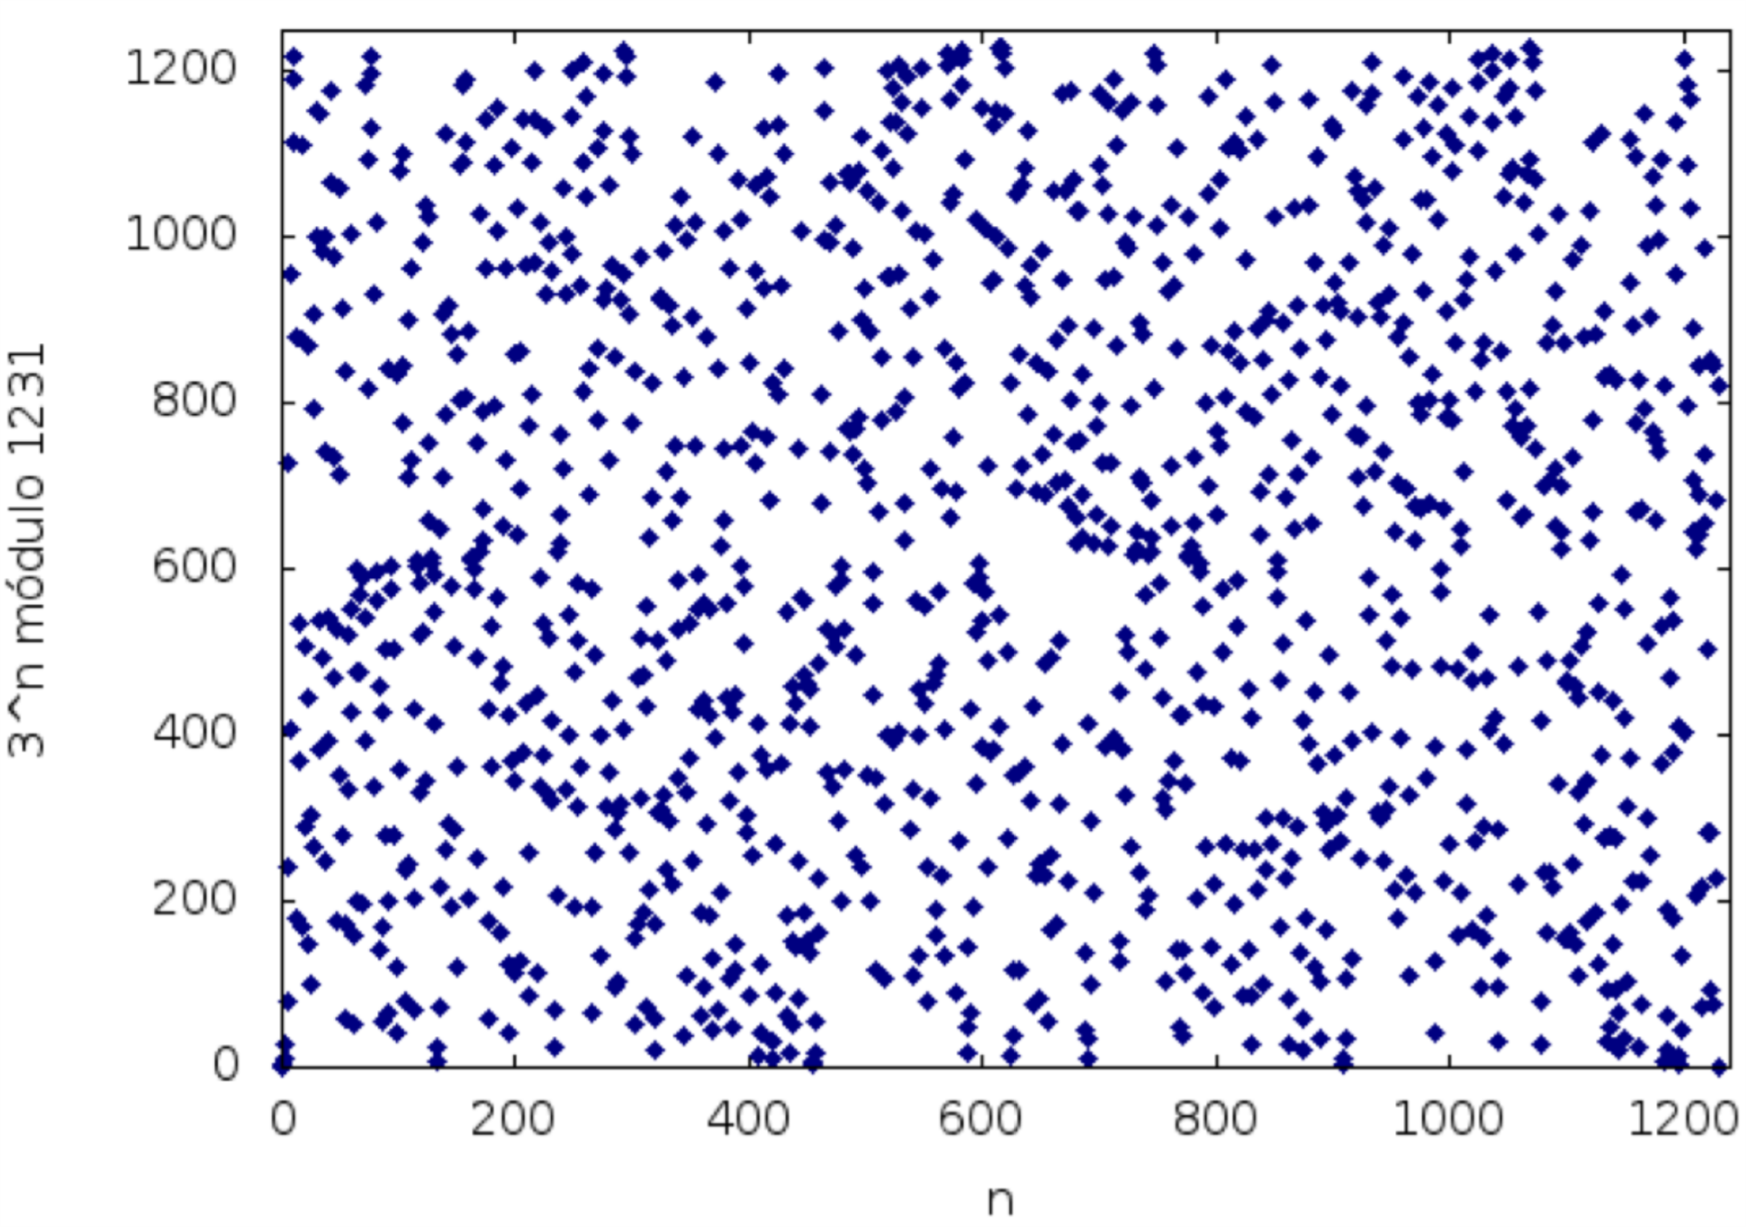
\includegraphics[width=\linewidth]{DL}
		\end{column}
		\begin{column}{0.5\textwidth}
			Discrete Logarithm with $G=\mathbb{Z}_{1231}$, $g=3$.
			
			\small{Adolfo Quirós Gracián. \textit{Grupos y criptografía: de Julio César a las curvas elípticas.}}
		\end{column}
	
	\end{columns}


\end{frame}


\begin{frame}{Complexity classes}

\begin{block}{Definition (Class P)}
	The set of decision problems which can be solved in polynomial time.
\end{block}

\begin{block}{Definition (Class NP)}
	The set of decision problems where a $True$ answer can be verified in polynomial time, given some extra information (certificate).
\end{block}
	
\end{frame}



\begin{frame}{Complexity classes}

\begin{block}{Definition (Polynomial-time reduction $L_1 \leq_P L_2$)}
	Be $L_1$ and $L_2$ two decision problems. $L_1$ can be reduced in polynomial time to $L_2$ if $L_1$ can be solved using $L_2$ as a subroutine plus a polynomial time.
\end{block}

\begin{block}{Definition (Class NP-complete or NPC)}
	A decision problems $L$ is in \textbf{NPC} if:
	\begin{enumerate}
		\item $L \in $ \textbf{NP}, and
		\item $L_1 \leq_P L \quad \forall L_1 \in $ \textbf{NP}.
	\end{enumerate}
\end{block}
\end{frame}


\section{Residuos Cuadráticos}

\begin{frame}{Residuos Cuadráticos}
	\begin{definition}
		Sea $x\in \mathbb{Z}^*_n$. Se dice que $x$ es un \textit{residuo cuadrático}
		módulo n, o un \textit{cuadrado} módulo n, si existe un $a \in \mathbb{Z}^*_n$
		tal que
		
		$x \equiv a^2 \, mod \, n$.
		
		Si no existe dicho $a$, entonces $x$ se llama un \textit{no-residuo cuadrático} módulo n.
	\end{definition}

	Al conjunto de los residuos cuadráticos módulo n los denotaremos como $Q_n$.
	Al de los no-residuos cuadráticos, como $\overline{Q_n}$.
\end{frame}


\begin{frame}{Residuos Cuadráticos}
	\begin{example}
		Si tomamos $n=4$, los no-residuos cuadráticos son $2$ y $3$, y el único residuo cuadrático es $1$:
		\begin{align*}
		1^2 \equiv 1 \, mod \, 4 \qquad 2^2 \equiv 0 \, mod \, 4 \qquad  3^2 \equiv 1 \, mod \, 4
		\end{align*}
	\end{example}
	Por definición $0 \notin \mathbb{Z}^*_n$, y por tanto $0 \notin Q_n$ ni $0 \notin \overline{Q_n}$.
\end{frame}

\begin{frame}{Residuos Cuadráticos: Propiedades}
	\begin{block}{Proposición}
		Sea $p>1$ un n\'umero primo, entonces $|Q_p| = |\overline{Q_p}| = \frac{p-1}{2}$.
	\end{block}
	\begin{block}{Proposición}
		Sea $n$ y $m$ dos n\'umeros enteros positivos coprimos. Entonces un elemento
		$x \in {\mathbb Z}_{mn}$ es un residuo cuadr\'atico si y s\'olo si $x~mod~m$
		y $x~mod~n$ son residuos cuadr\'aticos en ${\mathbb Z}_m$ y ${\mathbb Z}_n$
		respectivamente.
		
		Adem\'as, si $a$ y $b$ son ra\'ices cuadradas de $x~mod~m$ y $x~mod~n$ en sus
		correspondientes anillos, podemos combinarlas mediante el Teorema Chino de los Restos
		para obtener una ra\'iz cuadrada de $x$ en ${\mathbb Z}_{mn}$.
		
		En particular, esto es cierto cuando queramos estudiar los residuos cuadr\'aticos en
		${\mathbb Z}_{pq}$ con $p$ y $q$ dos primos impares distintos, que son en particular coprimos.
	\end{block}
	\begin{corollary}
		Sea $n = pq$ el producto de dos primos distintos, entonces el n\'umero de residuos cuadr\'aticos m\'odulo $n$ es $\frac{(p-1)(q-1)}{4}$.
	\end{corollary}
\end{frame}


\begin{frame}{Residuos Cuadráticos: Símbolo de Legendre}
	\begin{definition}[Símbolo de Legendre]
		Dados un primo impar $p$ y un entero $a$, se define el {\em Símbolo de Legendre} como
		
		\begin{center}
			$
			\left( \dfrac{a}{p} \right) =
			\begin{cases}
			0, & si\ a \equiv 0 \, mod \, p\\
			1, & si\ a \in Q_p  \\
			-1, & si\ a \in \overline{Q_p} \\
			\end{cases}
			$
		\end{center}
	\end{definition}
\end{frame}


\begin{frame}{Residuos Cuadráticos: Símbolo de Jacobi}
	\begin{definition}[Símbolo de Jacobi]
		Sea $n$ un entero impar positivo cuya descomposici\'on en factores primos es $n = p_1^{e_1} p_2^{e_2} \cdots p_r^{e_r}$ y sea $a$ un entero. Entonces definimos
		el \textit{s\'imbolo de Jacobi} de $a$ y $n$ como
		\[\left( \dfrac{a}{n} \right) = \left( \dfrac{a}{p_1} \right)^{e_1} \cdot \left( \dfrac{a}{p_2} \right)^{e_2} \cdot \cdots \cdot \left( \dfrac{a}{p_t} \right)^{e_t}\]
	\end{definition}
	\begin{alertblock}{Observación}
		Un Símbolo de Jacobi $-1$ nos indica \textit{no-residuo}, pero un $1$ ya no indica necesariamente \textit{residuo cuadrático}.
	\end{alertblock}
\end{frame}

% TODO: reducir a FACT

\begin{frame}{Residuos Cuadráticos: Problema QR}
	\begin{description}[Parámetros]
		\item[Nombre] Problema de los residuos cuadr\'aticos (QR).
		\item[Parámetros] $N$ un entero impar tal que $N = pq$ para $p$ y $q$ primos, y el entero $x$ tal que $\left( \frac{x}{N} \right) = 1$.
		\item[Pregunta] ¿Es $x$ un residuo cuadrático en ${\mathbb Z}_N$?
	\end{description}
\end{frame}


\section{Pruebas Interactivas}

\begin{frame}{Pruebas Interactivas}

\begin{description}[Q]
	\item[Probador (P)] computacionalmente \textit{todopoderosa}.
	\item[Verificador (V)] cómputo limitado, probabilístico de tiempo de polinomial.
\end{description}

\end{frame}

\begin{frame}{Pruebas Interactivas}
	\begin{definition}[Sistema de Prueba Interactiva]
		
		Un problema de decisión $Q$ tiene un \textit{sistema de prueba interactiva} si tiene un protocolo de interacción polinomialmente acotado en número de mensajes que cumple:
		
		\begin{itemize}
			\item \textit{Completitud} Para toda instancia $q$ $Verdadera$, del problema $Q$, V acepta $q$ como $Verdadera$.
			\item \textit{Robustez} Para cada instancia $q$ $Falsa$, V rechaza la prueba de $q$ con una probabilidad no menor que $\epsilon = 1-n^{-c}$, para cualquier constante $c>0$ y donde $n$ es el tamaño de la instancia.
		\end{itemize}
		
	\end{definition}
\end{frame}


\begin{frame}{Pruebas Interactivas}


\begin{definition}
	Denominamos clase de problemas \textbf{IP} (Interactivos en tiempo Polinomial) al conjunto de problemas de decisión para los que existe un sistema de prueba interactivo.
\end{definition}


\end{frame}



\begin{frame}{Pruebas Interactivas}
	\begin{theorem}
		\textbf{NP} $\subset$ \textbf{IP}.
	\end{theorem}
	
	\begin{proof}
		Sea $Q$ un problema \textbf{NP}. Definimos el siguiente protocolo:
		\begin{enumerate}
			\item  P resuelve la instancia del problema gracias a su capacidad de cómputo ilimitada y genera el certificado para V.
			\item  V recibe y verifica el certificado en tiempo polinomial. Si es válido, V acepta como $Verdadera$ la instancia. Si no, rechaza la prueba.
		\end{enumerate}
		%El protocolo es completo y robusto, con probabilidad nula de falso positivo, pues si la instancia es $Falsa$, ningún P puede generar un certificado que no existe.
	\end{proof}
\end{frame}




\begin{frame}{Ejemplo Pruebas Interactivas: Problema QR}
	\begin{theorem}
		El problema QR tiene un sistema de prueba interactivo.
	\end{theorem}

	\begin{description}[Parámetros]
		\item[Nombre] Problema de los residuos cuadr\'aticos (QR).
		\item[Parámetros] $N$ un entero impar tal que $N = pq$ para $p$ y $q$ primos, y el entero $x$ tal que $\left( \frac{x}{N} \right) = 1$.
		\item[Pregunta] ¿Es $x$ un residuo cuadrático en ${\mathbb Z}_N$?
	\end{description}
\end{frame}


\begin{frame}{Ejemplo Pruebas Interactivas: Problema QR}
\begin{block}{Prueba interactiva para QR $(x,N)$}
	
	Sea $t(n)$ un polinomio en $n$, el tamaño de la instancia $(x,N)$. P y V repiten $t(n)$ veces los siguientes pasos.
	
	\begin{enumerate}
		
		\item P $\rightarrow$ V :\quad $u \in_R \mathbb{Z}^{Q+}_N$, \; un residuo cuadrático en $\mathbb{Z}_N$.
		
		\item V $\rightarrow$ P :\quad $b \in_R \{0,\,1\}$.
		
		\item P $\rightarrow$ V :\quad $w$,\; una raíz cuadrada aleatoria de $u\cdot x^b$.
		
		\item V comprueba si:
		\[
		w^2 \overset{?}{\equiv}
		\begin{cases}
		u\, mod\, N, & si\ b = 0\\
		xu\, mod\, N, & si\ b = 1.\\
		\end{cases}
		\]
		
		Si la comparación falla, V termina en rechazo. En caso contrario, vuelve al paso 1.
		
	\end{enumerate}
	
\end{block}

% TODO : en las diapositivas extra
% TODO: para la presentación, si preguntan por qué t(n) depende del tamaño de la entrada, preparar ejemplo de Z_5 o Z_15 mejor, por 15=3*5 los primos impares, indicar que hay 7 residuos cuadráticos y 7 no-residuos, que la cantidad de u's distintos que puede tomar aleatoriamente de entre los rq y los no-rq para intentar engañarlo es mínima, y en pocas iteraciones pueden haber probado todas las combinaciones, y seguir el protocolo es repetir valores ya contrastados, y comparando con primos de 2048 bits, se pueden pedir más iteraciones.
\end{frame}


\begin{frame}{Ejemplo Pruebas Interactivas: Problema QR}
	\begin{proof}
		La prueba es \textbf{completa}:
		
		Instancia $(x,N)$ $Verdadera$ $\Rightarrow$ $x$ es residuo cuadrático, existe raíz.
		
		P computacionalmente todopoderoso $\Rightarrow$ puede calcular $w$ raíz de $x$ o $xu$.
		
		V acepta la prueba de P.
	\end{proof}
\end{frame}

\begin{frame}{Ejemplo Pruebas Interactivas: Problema QR}
\begin{proof}
	La prueba es \textbf{robusta}:
	
	Instancia $Falsa$, $x$ no residuo cuadrático.
	P$^*$ intenta adivinar el reto $b\in_R\{0,1\}$.
	\begin{itemize}
		\item Si $b=0$, sigue el protocolo, elige $u \in_R \mathbb{Z}^{Q+}_N$.
		
		\item Si $b=1$, elige $u \equiv x^{-1} a^2 \, mod \, N$, con $a \in_R \mathbb{Z}_N$.
		Responde con $w = a$.		
		V comprobará $w^2\equiv a^2 \overset{?}{\equiv} x\cdot x^{-1} a^2 \equiv a^2 \, mod \, N$.
	\end{itemize}

	Si P$^*$ falla al adivinar, o no existirá raíz de $xu$, o $w^2 \not \equiv u \, mod \, N$.
	
	Probabilidad de acertar el reto $b$: $\frac{1}{2}$.
	
	Probabilidad de pasar la prueba: $2^{-t(n)}$.
	
\end{proof}
\end{frame}



\section{Pruebas de Conocimiento Cero}

\begin{frame}{Pruebas de Conocimiento Cero}
	
\end{frame}

\end{document}